\onecolumn

\appendix

\begin{appendices}

\section{Output from LLM agents}
\label{app:agent_output_schema}
\lstdefinestyle{XMLStyle}{
  language=XML,
  basicstyle=\ttfamily\small,
  numbers=left,
  numberstyle=\tiny,
  stepnumber=1,
  numbersep=5pt,
  tabsize=2,
  extendedchars=true,
  breaklines=true,
  keywordstyle=\color{blue},
  stringstyle=\color{orange},
  commentstyle=\color{green},
  morestring=[b]",
  showspaces=false,
  showtabs=false,
  showstringspaces=false
}
This document presents the output structure from an LLM (Large Language Model) agent's code review. Each field in the structure has a specific significance:

\begin{itemize}
    \item \textbf{description}: Provides a detailed explanation of the issue or suggestion identified by the LLM agent.
    \item \textbf{corrective\_code}: Contains the proposed code changes or additions to address the identified issue (if any).
    \item \textbf{file\_path}: Indicates the specific file where the issue was found or where changes should be applied.
    \item \textbf{line\_number}: Specifies the exact line in the file where the issue occurs or where changes should be made.
    \item \textbf{confidence\_score}: Represents the LLM agent's confidence level in its assessment or suggestion.
    \item \textbf{bucket}: Categorizes the type of issue or suggestion (e.g., Readability, Performance optimization, Business requirement adherence, Documentation etc.).
\end{itemize}

\section*{LLM Agent Review Output}

\begin{lstlisting}[style=XMLStyle]
<review>
  <comments>
    <comment>
      <description></description>
      <corrective_code></corrective_code>
      <file_path></file_path>
      <line_number></line_number>
      <confidence_score></confidence_score>
      <bucket></bucket>
    </comment>
  </comments>
</review>
\end{lstlisting}



\section{Capabilities}
\label{app:capabilities}
\subsection{Contextual code reviews}
DeputyDev's core feature is to perform highly contextual code review and provide in-line comments indicating issues or potential improvements. \ref{fig:dd_comm_security} \ref{fig:dd_comm_story} \ref{fig:dd_comm_maint}

\subsection{Context-aware chatting}
DeputyDev users can perform context-aware chatting with it. This is a specifically useful feature which can act as a learning companion. This feature can be used for generating code, tests, docstrings and much more. The feature is initialized by starting the comment with \texttt{\#dd} prefix \ref{fig:dd_param_query} \ref{fig:dd_docstring}

\subsection{PR summary}
DeputyDev generates PR summary along with sizing and review time estimates. This feature is specifically helpful for reviewers and service owners to get a gist of the change without actually going through the diff. \ref{fig:dd_comm_summary}

\begin{figure*}[htbp]
    \centering
    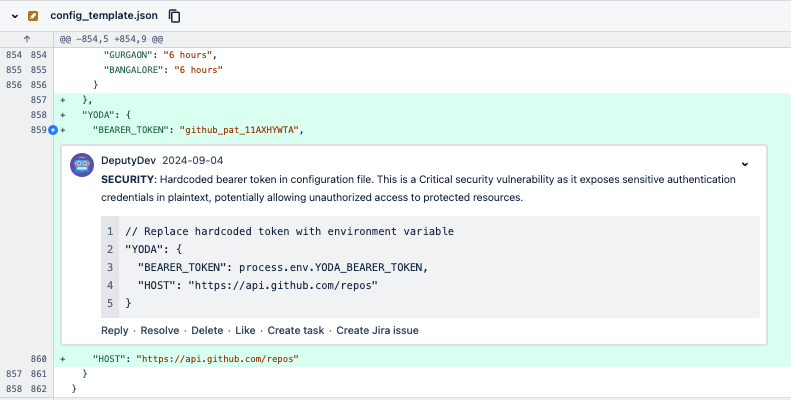
\includegraphics[scale=0.40]
    {Figures/dd_comm_security.png}
    \caption{DeputyDev chatting can be used as a learning companion. It can help out developers and reviewers know of best practices and how to implement them.}
    \label{fig:dd_comm_security}
\end{figure*}

\begin{figure*}[htbp]
    \centering
    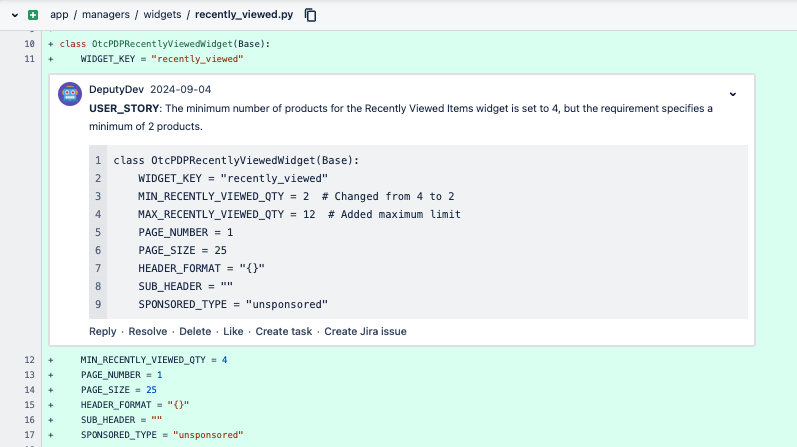
\includegraphics[scale=0.40]
    {Figures/dd_comm_story.png}
    \caption{DeputyDev acts as a powerful tool to generate docstrings and documentations.}
    \label{fig:dd_comm_story}
\end{figure*}

\begin{figure*}[htbp]
    \centering
    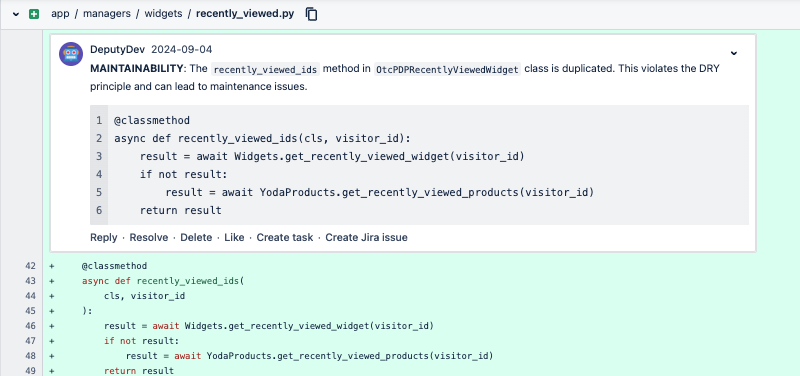
\includegraphics[scale=0.40]
    {Figures/dd_comm_maint.png}
    \caption{DeputyDev acts as a powerful tool to generate docstrings and documentations.}
    \label{fig:dd_comm_maint}
\end{figure*}

\begin{figure*}[htbp]
    \centering
    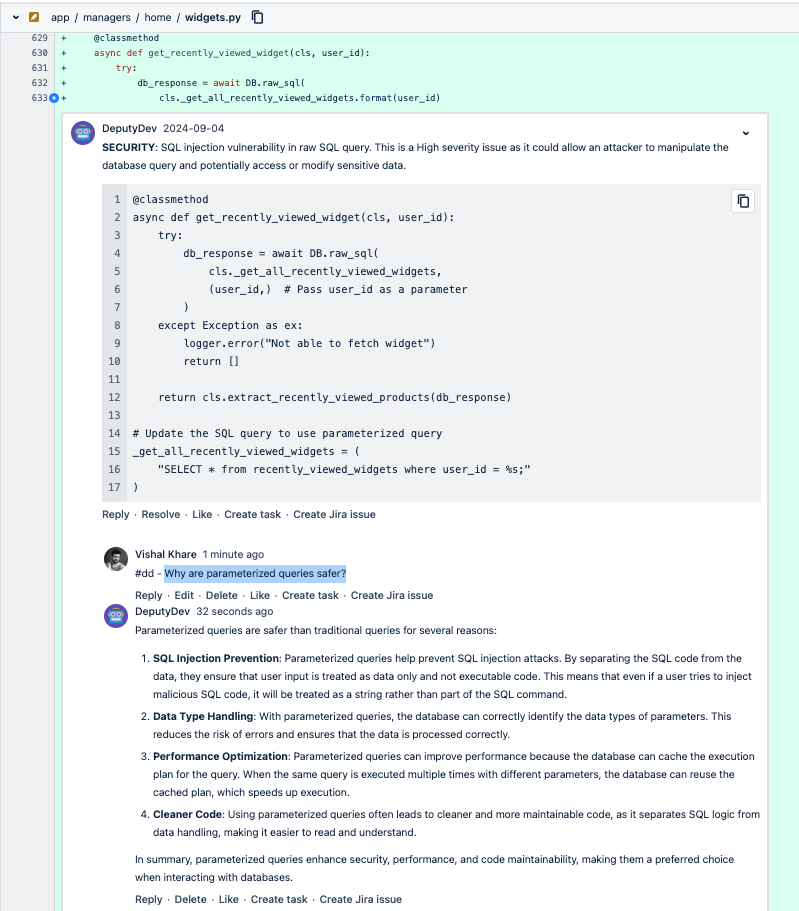
\includegraphics[width=0.8\textwidth]
    {Figures/dd_param_query.png}
    \caption{DeputyDev chatting can be used as a learning companion. It can help out developers and reviewers know of best practices and how to implement them.}
    \label{fig:dd_param_query}
\end{figure*}

\begin{figure*}[htbp]
    \centering
    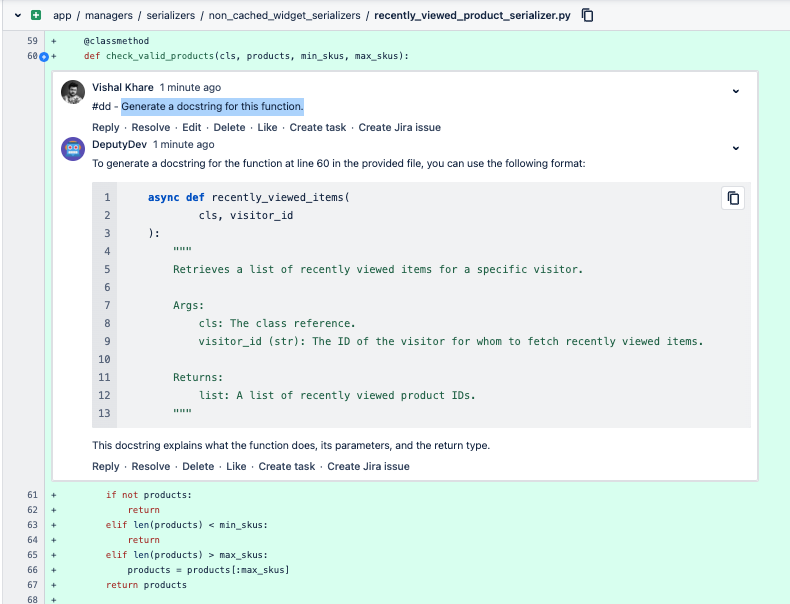
\includegraphics[scale=0.40]
    {Figures/dd_docstring.png}
    \caption{DeputyDev acts as a powerful tool to generate docstrings and documentations.}
    \label{fig:dd_docstring}
\end{figure*}

\begin{figure*}[htbp]
    \centering
    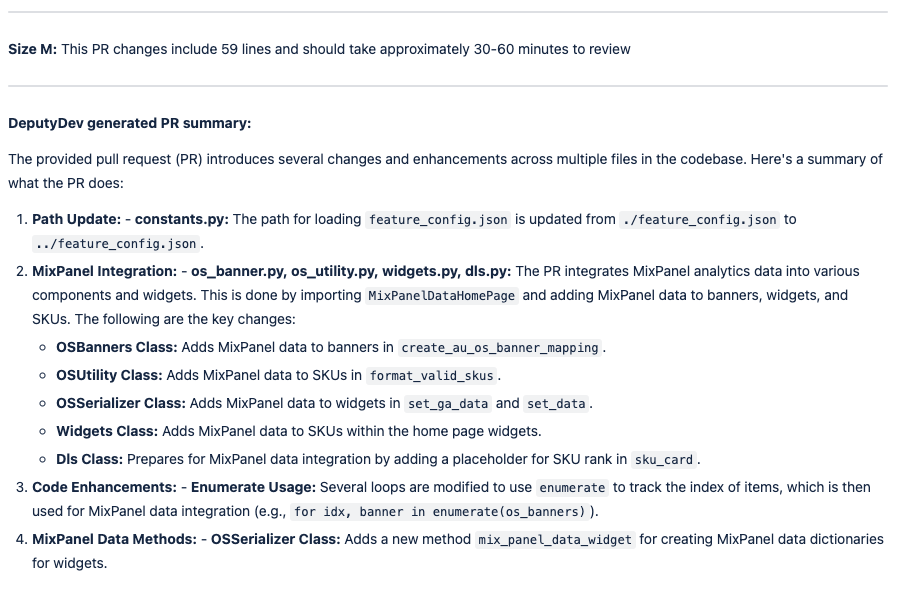
\includegraphics[scale=0.50]
    {Figures/dd_comm_summary.png}
    \caption{DeputyDev generated PR summary}
    \label{fig:dd_comm_summary}
\end{figure*}

\section{Mathematical calculations}
\label{app:calculations}

\subsection*{1. Average code review time}

\begin{equation}
\mathlarger{\mathlarger{\text{Average code review time} = \frac{\sum_{i=1}^{n} \text{code review time}_i}{n}}}
\end{equation}

Where $n$ is the total number of pull requests.

\subsection*{2. Average code review time per LOC (Lines of Code)}

\begin{equation}
\mathlarger{\mathlarger{\text{Average code review time per LOC} = \frac{\sum_{i=1}^{n} \frac{\text{code review time}_i}{\text{lines of code}_i}}{n}}}
\end{equation}

\subsection*{3. Median code review time}

\begin{equation}
\mathlarger{\mathlarger{
\text{Median code review time} = 
\begin{cases}
    x_{\frac{n+1}{2}}, & \text{if $n$ is odd} \\[2ex]
    \frac{x_{\frac{n}{2}} + x_{\frac{n}{2}+1}}{2}, & \text{if $n$ is even}
\end{cases}
}}
\end{equation}

Where $x_1, x_2, ..., x_n$ are the sorted code review times in ascending order.
\end{appendices}